\documentclass{article}
\usepackage{fancyhdr}
\usepackage{tikz}
\pagestyle{fancy}
\setlength{\headheight}{35pt}
\lhead{Distributed System I\\Wintersemester2020/21\\Assignment 1}
\chead{}
% bfseries
\rhead{Ciheng Zhang (3472321)\\Chenxi Li(3502796)\\Yaosheng Zheng (3563285)\\Leqi Xu(3556962)}
\cfoot{\thepage}
\renewcommand{\headrulewidth}{0.4pt}

\begin{document}
\begin{titlepage}
    \title{\Huge \textbf{Distributed System I\\Wintersemester2020/21\\Assignment 1} }
    \author{\LARGE \textsl{Ciheng Zhang (3472321) zch3183505@gmail.com}\\\LARGE \textsl{Chenxi Li(3502796) cli216@outlook.com }\\\LARGE \textsl{Leqi Xu(3556962) st176119@stud.uni-stuttgart.de} \\\LARGE \textsl{Yaosheng Zheng (3563285) zhengyaosheng312@icloud.com}\\\LARGE \textsl{Team 19 } \\[200pt]}
    \date{\today}
    \maketitle
    \thispagestyle{empty}
\end{titlepage}
\newpage
\section*{Transparency Levels}
\subsection*{a)}
Concurrency transparency: in this question we use http protocol. HTTP allow Allow multiple people to access at the same time.\\
\\Replication transparency: here users never know how many copies exist in the server.\\
\\Scaling transparency: The server can extend the storage of the server but dont need to change the structure.
\subsection*{b)}
Concurrency transparency, Replication transparency, Scaling transparency. The reason is same as the question a because of http protocol.
\\
\\Location transparency: In the question we use domian not IP address. we need to use DNS to got the real address of the server.So we actually dont know where its the server.\\
\\Migration transparency: we use DNS to locate. So if we change our real location of our server, there will be no affect to application.
\subsection*{c)}
We use write all and read one methode. 
\\Write operation: the protocol lock all copys. Then the client write the change to all copys. Then all lock release.
\\Read operation: At first lock all copys, and then the client read only one copy. after reading the locks release.
\\In this protocal the changes will be write in all the copys. And when the client is reading one copy.the server is locked no one can change the copys. so
it ensure delivers the most recent copy.
\section*{System Models}
\subsection*{a)}
In this question, The necessary assumptions are:  there is no Failure in the system(No communication Failure and no Process Failure). This mean if a requset is sent, after a period of time P2 always will recived it.
\subsection*{b)}
The transmission delay and excute time is always less than a $t_{max}$,also the drift of reciver and sender should be same.
\subsection*{c)}
Both P1 and P2 w.r.t a real time, and after the requset can be reached anyway. Justify: a requset is send and the transmission need some time. So $t_{P2}^{recive}(m_{req})$ and $t_{P1}^{send}(m_{req})$ must have a time delay. and we want to compare this two time. We need to make the tow local clock with reference with a same global time.
\subsection*{d)}
The P2 process  after process send responses in order recived, that can make $t_{P1}^{recive}(m_{res1})<t_{P1}^{recive}(m_{res2})$
and the P2 send responses of first msg after send second msg from P1. So $t_{P1}^{send}(m2)-t_{P1}^{send}(m1)<t_{delay}+t_{excution}+t_{drift}$.This mean the time between P1 send first message and second message should less than the send delay time and excution time in P2 and drift time of P2.

\section*{Three-Army-Problem}
\subsection*{a)}
The assumptions is there should be no Failure in communication, this mean all the message can always send to the reciver. also the delay time between send and recive should not be too long($d>k$).\\
Three army in the same time send the number of division. And then the largest send message to other 2 divisions about the attack time. Then at the attack time the largest division attack, after k mins the second-largest attack. And k mins later the smallest division attack.
\subsection*{b)}
\begin{tikzpicture}[scale=0.8]
    %时间线
    \draw[->](-3,3)--(10.5,3);
    \draw[->](-3,2)--(10.5,2);
    \draw[->](-3,1)--(10.5,1);
    %指向其他两个部队的线
    \draw[-latex,color=blue](-1,3)--(1,2);
    %\draw[-latex](-1,3)--(1,1);

    \draw[-latex,color=blue](-3,2)--(-1,3);
    \draw[-latex,color=blue](-3,2)--(-1,1);

    %\draw[-latex,color=purple](-1,1)--(1,3);
    \draw[-latex,color=blue](-1,1)--(1,2);
    %发起进攻的时间信息发送
    \draw[-latex](1,2)--(3,3);
    \draw[-latex](1,2)--(3,1);
    %绘制每个时间点虚线
    \draw[dotted,color=red,line width=2pt](-3,4)--(-3,0);
    \draw[dotted,color=red,line width=2pt](-1,4)--(-1,0);
    \draw[dotted,color=red,line width=2pt](1,4)--(1,0);
    \draw[dotted,color=red,line width=2pt](3,4)--(3,0);
    \draw[dotted,color=red,line width=2pt](4,4)--(4,0);
    \draw[dotted,color=red,line width=2pt](7,4)--(7,0);
    \draw[dotted,color=red,line width=2pt](10,4)--(10,0);
    %\draw[dotted,color=red,line width=2pt](-0.5,4)--(-0.5,0);
    %\draw[dotted,color=red,line width=2pt](7,4)--(7,0);
    %绘制开始进攻
    \draw[fill=blue](4,3) circle(0.1);
    \draw[fill=blue](7,2) circle(0.1);
    \draw[fill=blue](10,1) circle(0.1);
    %打标签
    \node at (-2.8,3.5){t0};
    \node at(-0.5,3.5){d+t0};
    \node at(1.5,3.5){2d+t0};
    \node at(3.5,3.5){3d+t0};
    \node at(5,3.5){2d+t0+k};
    \node at(8,3.5){2d+2k+t0};
    \node at(11,3.5){2d+3k+t0};
    \node at(-3.5,3){div1};
    \node at(-3.5,2){div2};
    \node at(-3.5,1){div3};
    \node at(7,0){Blue point: attack};
\end{tikzpicture}
in this diagram. we assum the largest division is div1 and second-largest is div 2 and smallest is div3.At time t0 div2 want to attack, and send message to div1 and div2. Then at time d div1 and div2 got the message and send back message about their size to div2. At 2d time div2 know all three divisions size, and send to div1 and div3 message about attack time. At 2d+t0+k time the bigest div1 start attack. After k time div2 and then div3. 

\section*{System Availablity}
\subsection*{a)}
\[A_X=\frac{60}{100}=0.6\]
\[A_Y=\frac{80}{100}=0.8\]
\subsection*{b)}
\[A_{DS}=1-\bar{A_X}\bar{A_Y}=0.92\]
\subsection*{c)}
\[P(X=up|Y=up)=\frac{60}{80}=0.75\]
\[P(X=up|Y=down)=0\]
\subsection*{d)}
accroding question c. if Y fail X must be fail:
\[P=1-0.2=0.8\]
\end{document}
